\documentclass[a4paper,12pt]{article}
\usepackage{titling}
\usepackage[utf8]{inputenc}
\usepackage{graphicx}
\usepackage{amsmath}
\usepackage{amssymb}
\usepackage{cleveref}
\usepackage{siunitx}
\usepackage{listings}
\usepackage[framed,numbered]{matlab-prettifier}
\usepackage{xcolor}
\usepackage{lipsum} % For generating filler text
\usepackage{float} % For controlling float placement
\usepackage{caption} % For custom captions

% Aliases
\newcommand{\Hz}[1]{%
    \ifcase#1
        \relax
    \or
        \,\text{Hz}
    \or
        \,\text{kHz}
    \or
        \,\text{MHz}
    \or
        \,\text{GHz}
    \else
        \,\text{Invalid}
    \fi
}


\title{%
  EE458L Lab 10 \\
  \large Nyquist Sampling Theorem
  }

\begin{document}

\author{Erik Chavarin \\ 823739365}
\date{November 6, 2023}

\maketitle
\section*{Introduction}
This lab is an exercise in understanding the Nyquist-Shannon sampling theorem given the Nyquist criterion in \cref{eq:NSST}.

\begin{equation}
    F_s > 2B
    \label{eq:NSST}
\end{equation} 

For a signal with bandwidth $B$, the criterion in \cref{eq:NSST} states that the sampling rate, $F_s$, must be a frequency that is over twice that of the highest frequency component in the signal to be sampled to allow for perfect reconstruction. In other words, $F_s$ must exceed the Nyquist rate $2B$. Another important concept from this criterion is the Nyquist frequency. The Nyquist frequency can be derived from \cref{eq:NSST} as shown in \cref{eq:NF}.

\begin{equation}
    F_{Ny} = \frac{F_s}{2} > B
    \label{eq:NF}
\end{equation} 

The Nyquist frequency is the highest frequency component able to be perfectly reconstructed from a given $F_s$. Violating the Nyquist criterion results in the distortion of the frequency components of a signal that are higher than $F_{Ny}$. In other words, a high frequency will erroneously manifest as a lower frequency in the sampling output.

With these concepts in mind, this lab investigates two sine waves sampled with two $F_s$ values, $F_{s1} = 48\Hz{2}$ and $F_{s2} = 8\Hz{2}$. The first sine wave, given in \cref{eq:x1}, has a frequency, $f_1 = 2\Hz{2}$ which passes the Nyquist criterion with both sampling rates. The second sine wave, given in \cref{eq:x2}, has a frequency, $f_2 = 6\Hz{2}$ which passes the Nyquist criterion with $F_{s1}$ but violates the Nyquist criterion with $F_s2$. 

\begin{equation}
    x_1(t) = sin(2 \pi t \cdot 2\Hz{2}) 
    \label{eq:x1}
\end{equation}

\begin{equation}
    x_2(t) = sin(2 \pi t \cdot 6\Hz{2}) 
    \label{eq:x2}
\end{equation}

The violation of the Nyquist criterion is evaluated by reconstructing (as much as possible) the continuous-time waveform by convolving the sampled signal with an interpolation kernel. The interpolation kernel is the impulse response of a low-pass filter (a sinc function) sampled at $F_{s1}$. 

In this report, the two sine wave signals, $x_1(t)$ and $x_2(t)$, will be investigated simultaneously (accounting for Task IV) so there will only be three tasks mentioned. All the scripting is performed in MATLAB R2022b.



\clearpage
\section*{Task I}
The investigation begins by sampling ten periods of \cref{eq:x1} and \cref{eq:x2} at $F_{s1}$. The sampling rate, $F_{s1}$, will not cause aliasing at the output because $F_{Ny}=24\Hz{2}$ is greater than both signals via \cref{eq:NF}. This sampling rate is also used as the reference time vector for when the signals are later sampled by $F_{s2}=8\Hz{2}$ in Task II. The two "unsampled" signals are shown in \cref{T1a} for $f_1=2\Hz{2}$ and \cref{T1b} for $f_2=6\Hz{2}$. The time vector has a length of $N_1 = f_1^{-1} \cdot 10 / F_{s1}^{-1} = 240$ for \cref{eq:x1} and $N_2 = f_2^{-1} \cdot 10 / F_{s1}^{-1} = 80$ for \cref{eq:x2}.

\begin{figure}[!h]
    \centering
    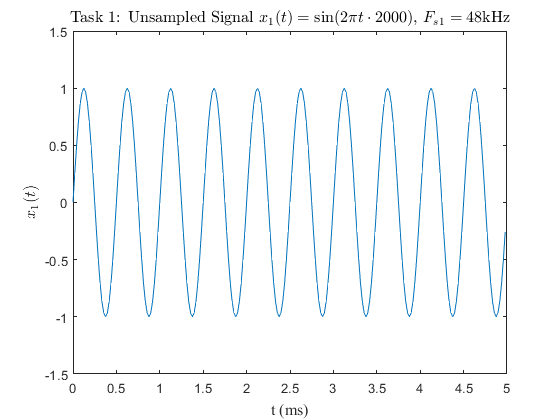
\includegraphics[width=1\textwidth]{T1a.png}
    \captionsetup{justification=centering}
    \caption{\small Ten cycles of \cref{eq:x1} using a time vector defined by $F_{s1}$ which gives a signal length of $N_1 = 240$.}
    \label{T1a}
\end{figure}

\begin{figure}[!t]
    \centering
    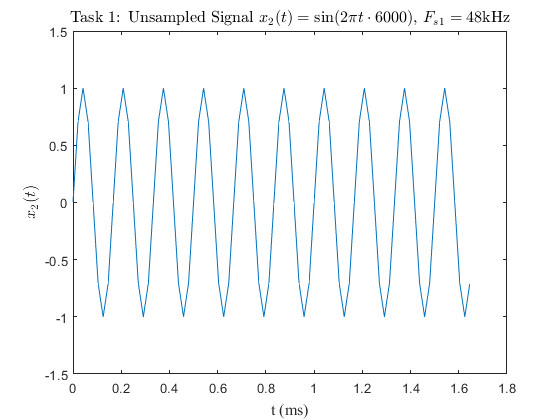
\includegraphics[width=1\textwidth]{T1b.png}
    \captionsetup{justification=centering}
    \caption{\small Ten cycles of \cref{eq:x2} using a time vector defined by $F_{s1}$ which gives a signal length of $N_2 = 80$.}
    \label{T1b}
\end{figure}



\clearpage
\section*{Task II}
Using the reference time vectors of length $N_1$ and $N_2$, a new time vector of equal length is obtained using $F_{s2}$. Because $F_{s2} = F_{s1}/6$, every sixth $T_{s1}$ sample of the original time vector is retained (i.e., $0T, 7T, 13T,$ etc.), and the other samples become zero. To implement this in MATLAB, the two signals were resampled at $F_{s2}$ creating a vector one-sixth the size $N_1$ and $N_2$, and then the signal elements were padded with zeros until the length was equal to the reference time vector length. Element-wise multiplication with a binary mask on the original time vector could've also been performed. The integer division of $N_2 / 6$ results in a signal vector of length $13$ so the resampled signal vector will have the last two samples either padded or truncated (as $13 \cdot 6 = 78$). In this case, they were truncated (the effect of this is spectral leakage in the frequency domain but the time domain signal---the relevant signal here---is unaffected).

The two resampled signals, $y_1(t)$ (of length $N_1$) and $y_2(t)$ (of length $N_2-2$), are shown in \cref{T2a} and \cref{T2b} respectively.

\begin{figure}[!h]
    \centering
    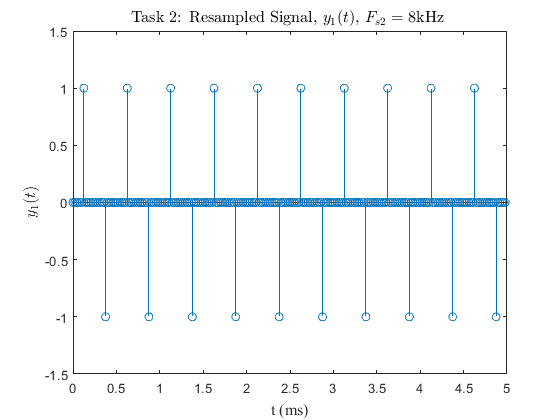
\includegraphics[width=1\textwidth]{T2a.png}
    \captionsetup{justification=centering}
    \caption{\small $x_1(t)$ signal vector of length $N_1$ resampled at $F_{s2}$, yielding $y_1(t)$. Every sixth sample in the reference time vector is retained and the rest are zero.}
    \label{T2a}
\end{figure}

\begin{figure}[!t]
    \centering
    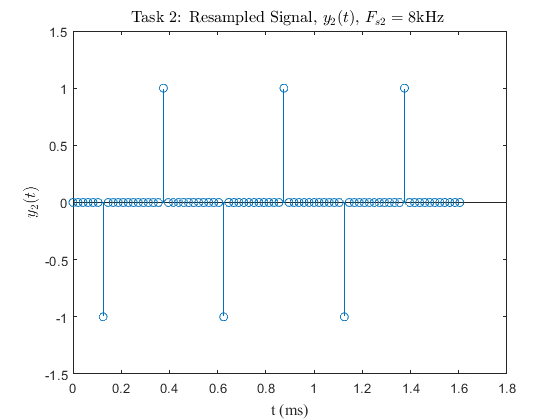
\includegraphics[width=1\textwidth]{T2b.png}
    \captionsetup{justification=centering}
    \caption{\small $x_2(t)$ signal vector of length $N_1$ resampled at $F_{s2}$, yielding $y_2(t)$. Every sixth sample in the reference time vector is retained and the rest are zero. The signal vector length is 78 instead of 80 because the integer division of 80 and 6 is 13. Therefore this signal is truncated compared to $x_2(t)$.}
    \label{T2b}
\end{figure}



\clearpage
\section*{Task III}
Both $y_1(t)$ and $y_2(t)$ are then convolved with an interpolation kernel, $g(t)$, to reconstruct the continuous-time signal (i.e., the resampled signal is passed through a lowpass filter). The Parks-McClellan algorithm is used via \texttt{firpm()} to implement an order 31 FIR lowpass filter with a $4\Hz{2}$ passband and $400\Hz{1}$ transition band sampled at $F_{s1}$. Due to the FIR nature of the interpolation kernel, it is not band-limited and therefore will not perfectly reconstruct the signals. However, the frequency of the sinusoid at the output will manifest and the effects of aliasing can be evaluated. The power spectrum of the FIR filter is shown in \cref{T3_filt}.

\begin{figure}[!h]
    \centering
    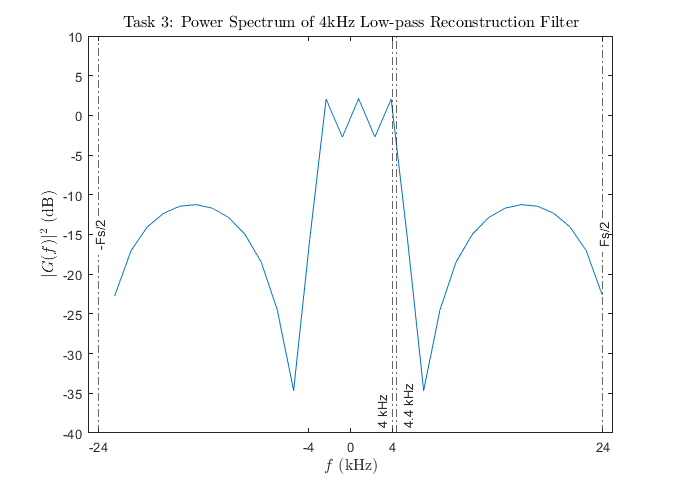
\includegraphics[width=1\textwidth]{T3_filt.png}
    \captionsetup{justification=centering}
    \caption{\small Power spectrum, $|G(f)|^2$, of the $N_{LP} = 31$ order Parks-McClellan FIR interpolation kernel, $g(t)$, sampled at $F_{s1}$. The specified passband, transition band, and Nyquist frequencies are labeled with dashed lines.}
    \label{T3_filt}
\end{figure}

The filter is applied using the \texttt{conv()} function to convolve $g(t)$ with $y_1(t)$ and $y_2(t)$. The resulting signals, $z_1(t)$ and $z_2(t)$, are shown in in \cref{T3a} and \cref{T3b} respectively. The output, $z_2(t)$ will experience aliasing because the requisite sampling rate must be $> 6\Hz{2} \cdot 2 = 12\Hz{2}$ via \cref{eq:NSST}. This is expected since $F_{Ny}$ for $F_{s2}$ (i.e., $F_{Ny2}$) is only $4\Hz{2}$ which is less than $f_2$. The Nyquist frequency is also referred to as the folding frequency because the remaining $2\Hz{2}$ outside $F_{Ny2}$ will "fold" back into the spectrum and experience modulo wrapping as the frequency increases. Therefore, the expected aliased output frequency is $f_2 \mod F_{Ny2} = 2\Hz{2}$.

\begin{figure}[!h]
    \centering
    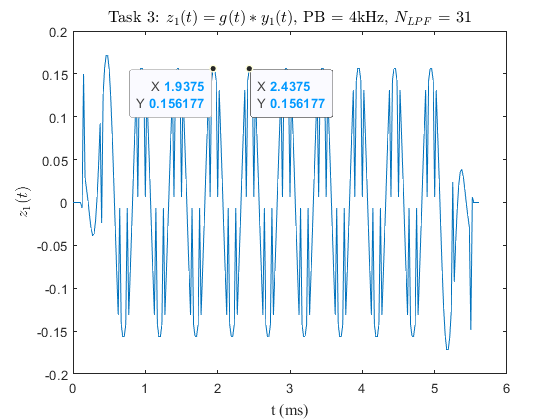
\includegraphics[width=1\textwidth]{T3a.png}
    \captionsetup{justification=centering}
    \caption{\small Reconstruction filter output, $z_1(t)$, of the resampled signal $y_1(t)$. Ten cycles are shown and the labeled data points demonstrate that the frequency is $(2.4375 - 1.9375)^{-1} = 2\Hz{2}$ indicating that no aliasing occurred as $f_1 = 2\Hz{2}$ for $y_1(t)$.}
    \label{T3a}
\end{figure}

\begin{figure}[!t]
    \centering
    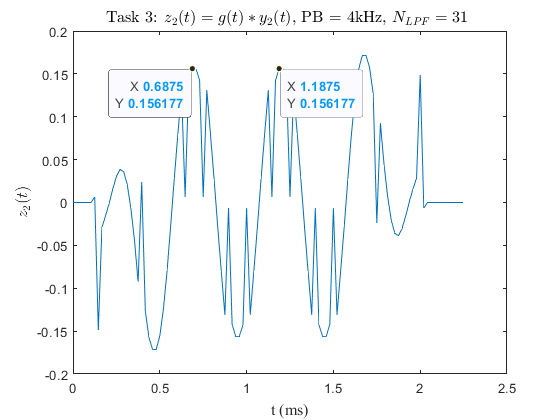
\includegraphics[width=1\textwidth]{T3b.png}
    \captionsetup{justification=centering}
    \caption{\small Reconstruction filter output, $z_2(t)$, of the resampled signal $y_2(t)$. Only three cycles are shown and the labeled data points demonstrate that the frequency is $(1.1875 - 0.6875)^{-1} = 2\Hz{2}$ indicating that aliasing \textit{has} occurred as $f_2 = 6\Hz{2} \neq 2\Hz{2}$ for $y_2(t)$. The $2\Hz{2}$ aliased output frequency exactly agrees with the modulo calculation performed above.}
    \label{T3b}
\end{figure}



\clearpage
\section*{MATLAB Script}
\definecolor{lightgray}{gray}{0.95}
\definecolor{mymauve}{rgb}{0.58,0,0.82}
\lstset{
    style              = Matlab-editor,
    basicstyle         = \ttfamily\small,
    backgroundcolor   = \color{lightgray},
    commentstyle      = \color{green!40!black},
    keywordstyle      = \color{blue},
    stringstyle       = \color{mymauve},
    numbers           = none, % Remove line numbering
    breaklines        = true,
    frame             = none, % Remove the frame
    framerule         = 0pt   % Remove the frame rule
}

\begin{lstlisting}

    % EE458L Lab 10
    % Erik Chavarin
    
    clear;
    close all;
    
    % Sampling freqs
    Fs1 = 48e3;
    Ts1 = Fs1^-1;
    Fs2 = 8e3;
    Ts2 = Fs2^-1;
    
    % Signal freqs (Tasks 1 & 4)
    fm1 = 2e3;
    Tm1 = fm1^-1;
    fm2 = 6e3;
    Tm2 = fm2^-1;
    
    % Time vector and resampled time vector
    % Task 1:
    t1 = 0:Ts1:Tm1*10-Ts1;
    t_resamp1 = 0:Ts2:Tm1*10-Ts2;  % Needed to produce resampled signal elements
    % Task 4:
    t2 = 0:Ts1:Tm2*10-Ts1;
    t_resamp2 = 0:Ts2:Tm2*10-Ts2; 
    % Vectors must begin at 0 to create a fiducial marker
    
    % Task 1: Signal generation
    % fm = 2 kHz
    x1 = sin(2 * pi * fm1 .* t1);
    x_resamp1 = sin(2 * pi * fm1 .* t_resamp1);
    % Task 4: fm = 6 kHz
    x2 = sin(2 * pi * fm2 .* t2);
    x_resamp2 = sin(2 * pi * fm2 .* t_resamp2);
    
    % Task 2: Signal resampling
    % Every [pad] zeros, an element from the resampled signal is inserted into 
    % the vector so length(x) == length(y), same time vector may be used
    pad = 6;  % T, 7T, 13T, ...
    y1 = zeros(1,pad*length(x_resamp1));
    y1(1:pad:end) = x_resamp1;
    % Task 4:
    y2 = zeros(1,pad*length(x_resamp2));
    y2(1:pad:end) = x_resamp2;  % 80/6 \approx 13
    % y2 = [y2, [0, 0]];  % Padding with two more zeros
    
    % Task 3: LPF applied to resampled signal
    %firpm LPF specs: 4 kHz pb + 400 Hz tb, Fs = 48 kHz
    pb = 4e3;  % passband width
    tb = 4e2;  % transition bandwidth
    fI = [0, pb, pb+tb, Fs1/2] / (Fs1 / 2);  % Normalized by Nyquist freq
    aI = [1, 1, 0, 0];  % LPF with full suppression on output
    N = 31;  % Order 31, firpm returns N+1 samples
    g = firpm(N, fI, aI);  % Impulse response
    G = fftshift(fft(g));  % Transfer function centered about DC
    fshift = (-N/2:N/2)*(Fs1/N);  % Symmetric spectrum axis
    
    
    z1 = conv(g, y1);
    z2 = conv(g, y2);
    t_conv1 = 0:Ts1:(Tm1*10+Ts1*N)-Ts1;
    t_conv2 = 0:Ts1:(Tm2*10+Ts1*N)-3*Ts1;  % Shave off a bit (because 80/6)
    % t_conv2 = 0:Ts1:(Tm2*10+Ts1*N)-Ts1;  % N = 80 (no shaving)
    
    % Plotting (Signals)
    sgtitle("Lab 10: Nyquist--Shannon Sampling Theorem", ...
        "FontSize", 14, "FontName", "Serif", "Interpreter", "latex")
    % x1
    subplot(2,3,1)
    plot(t1*1e3, x1)
    title("Task 1: Unsampled Signal $x_1(t) = \sin(2 \pi t \cdot 2000)$, " + ...
        "$F_{s1} = 48$kHz", "FontSize", 12, "FontName", "Serif", "Interpreter", ...
        "latex")
    xlabel("t (ms)", "FontSize", 12, "FontName", "Serif")
    ylabel("$x_1(t)$", ...
        "FontSize", 12, "FontName", "Serif", "Interpreter", "latex")
    ylim([-1.5,1.5]);
    
    subplot(2,3,2)
    stem(t1*1e3, y1)
    title("Task 2: Resampled Signal, $y_1(t)$, $F_{s2} = 8$kHz ", ...
        "FontSize", 12, "FontName", "Serif", "Interpreter", "latex")
    xlabel("t (ms)", "FontSize", 12, "FontName", "Serif")
    ylabel("$y_1(t)$", ...
        "FontSize", 12, "FontName", "Serif", "Interpreter", "latex")
    ylim([-1.5,1.5]);
    
    subplot(2,3,3)
    plot(t_conv1*1e3, z1)
    title("Task 3: $z_1(t) = g(t) * y_1(t)$, PB = 4kHz, $N_{LPF}$ = 31", ...
        "FontSize", 12, "FontName", "Serif", "Interpreter", "latex")
    xlabel("t (ms)", "FontSize", 12, "FontName", "Serif")
    ylabel("$z_1(t)$", ...
        "FontSize", 12, "FontName", "Serif", "Interpreter", "latex")
    
    % x2
    subplot(2,3,4)
    plot(t2*1e3, x2)
    title("Task 1: Unsampled Signal $x_2(t) = \sin(2 \pi t \cdot 6000)$, " + ...
    "$F_{s1} = 48$kHz", "FontSize", 12, "FontName", "Serif", "Interpreter", ...
        "latex")
    xlabel("t (ms)", "FontSize", 12, "FontName", "Serif")
    ylabel("$x_2(t)$", ...
        "FontSize", 12, "FontName", "Serif", "Interpreter", "latex")
    ylim([-1.5,1.5]);
    
    subplot(2,3,5)
    stem(t2(1:1:length(t2)-2)*1e3, y2)
    % stem(t2*1e3, y2)
    title("Task 2: Resampled Signal, $y_2(t)$, $F_{s2} = 8$kHz ", ...
        "FontSize", 12, "FontName", "Serif", "Interpreter", "latex")
    xlabel("t (ms)", "FontSize", 12, "FontName", "Serif")
    ylabel("$y_2(t)$", ...
        "FontSize", 12, "FontName", "Serif", "Interpreter", "latex")
    ylim([-1.5,1.5]);
    
    subplot(2,3,6)
    plot(t_conv2*1e3, z2)
    title("Task 3: $z_2(t) = g(t) * y_2(t)$, PB = 4kHz, $N_{LPF} = 31$ ", ...
        "FontSize", 12, "FontName", "Serif", "Interpreter", "latex")
    xlabel("t (ms)", "FontSize", 12, "FontName", "Serif")
    ylabel("$z_2(t)$", ...
        "FontSize", 12, "FontName", "Serif", "Interpreter", "latex")
    
    % Plotting (LPF)
    plot(fshift/1000, 20*log10(abs(G)))
    title("Task 3: Power Spectrum of $4$kHz Low-pass Reconstruction Filter", ...
        "FontSize", 12, "FontName", "Serif", "Interpreter", "latex")
    xlabel("$f$ (kHz)", ...
        "FontSize", 12, "FontName", "Serif", "Interpreter", "latex")
    ylabel("$|G(f)|^2$ (dB)", ...
        "FontSize", 12, "FontName", "Serif", "Interpreter", "latex")
    xticks([-24 -4 0 4 24])  % Plots frequency points of interest
    xline([-Fs1/2e3, Fs1/2e3], "-.", ["-Fs/2", "Fs/2"], ...
        LabelHorizontalAlignment="center", LabelVerticalAlignment="middle")
    
    % Label passband and transition band
    xline(pb/1e3, "-.", "4 kHz", ...
        LabelHorizontalAlignment="left", LabelVerticalAlignment="bottom")
    xline( (pb+tb)/1e3, "-.", "4.4 kHz", ...
        LabelHorizontalAlignment="right", LabelVerticalAlignment="bottom")
    ylim([-40, 10])

\end{lstlisting}



\section*{Conclusion}
A successful demonstration of the Nyquist-Shannon sampling theorem and aliasing was performed in this lab. I have had previous experience in undersampling signals in both python and MATLAB but this exercise was unique to me in two ways. Firstly, the signal vector size remained constant for sampling and resampling which didn't greatly affect the analysis but was a more practical implementation of a sampled signal and made the signal vectors more consistent. Secondly, in my previous exercises, I have never used a reconstruction filter to interpolate a sampled signal. While this was by no means a perfect reconstruction filter due to a finite impulse response, it was still insightful. I find aliasing to be a very interesting phenomenon and it was satisfying to see the modulo operation agree with the simulated filter output.



\end{document}
